%Latex2e file
\documentclass[12pt,letterpaper]{article}
%\renewcommand{\arraystretch}{2}
%\input{\scrload.tex}
\setlength{\textwidth}{6.5in}
\setlength{\textheight}{9.5in}

\setlength{\oddsidemargin}{-.25in}
\setlength{\evensidemargin}{-.25in}
\setlength{\topmargin}{-.25in}
\pagestyle{empty}

\usepackage{amsmath}
\usepackage{amssymb}
\usepackage{graphicx}

\newcommand{\R}{\ensuremath{{\mathbb{R}}}}
\newcommand{\Z}{\ensuremath{{\mathbb{Z}}}}
\newcommand{\Q}{\ensuremath{{\mathbb{Q}}}}
\newcommand{\N}{\ensuremath{{\mathbb{N}}}}
\newcommand{\C}{\ensuremath{{\mathbb{C}}}}
\newcommand{\Proof}{\noindent {\bf Proof: }}
\newcommand{\QED}{\begin{flushright}QED\end{flushright}}
\newcommand{\Refl}{{\bf Reflexive: }}
\newcommand{\Symm}{{\bf Symmetric: }}
\newcommand{\Tran}{{\bf Transitive: }}
\newcommand{\ep}{\varepsilon}
\newcommand{\ri}{\right|}
\newcommand{\lef}{\left|}
\newcommand{\toR}{\to \R}
\newcommand{\fancy}[1]{#1_{\text{fancy}}}
\newcommand{\pro}[1]{\noindent {\bf #1}}
\newcommand{\prob}[1]{\newpage\noindent {\bf #1}}
\newcommand{\bacon}{\approx}

   
\begin{document}
\begin{flushright}
Nick Kerner

Homework 5

Chapter 4: 1a, 10, 15, 19, 20a, 21, 28 (only the part where you ``prove that if one pair of opposite
sides has this property, then so does the other pair of opposite sides''.)
Chapter 5
9 (Compare with \#19 in Ch. 4)

\end{flushright}
\begin{center}
\large{Geometry}\\
\end{center}

\pro{1a} State the converse to Euclid V.  Prove this converse as a proposition in neutral geometry.\\

Converse of Euclidean parallel postulate: Given two lines intersected by a transversal.  If the two lines meet on one side of the transversal, then the two lines are intersected by the transversal in such a way that the sum of the degree measures of the two interior angles on one side of the transversal is less than $180^\circ$.\\


\Proof

Given two lines m and l and a transveral t such that m and l meet on one side of the transversal, let A be the point where t intersects m, B be the point where t intersects l, and C be the point where m intersects l. \\

Notice that this constructs $\triangle ABC$.  By corollary 2 to the External angle theorem we know that the sum of the degree measures of any two angles of a triangle is less than $180^\circ$.  Therefore $(\angle A)^\circ + (\angle B)^\circ \leq 180$.  Therefore we know that the two lines are intersected by the transversal in such a way that the sum of the degree measures of the two interior angles on one side of the transversal is less than $180^\circ$, so we are done.

\begin{center}
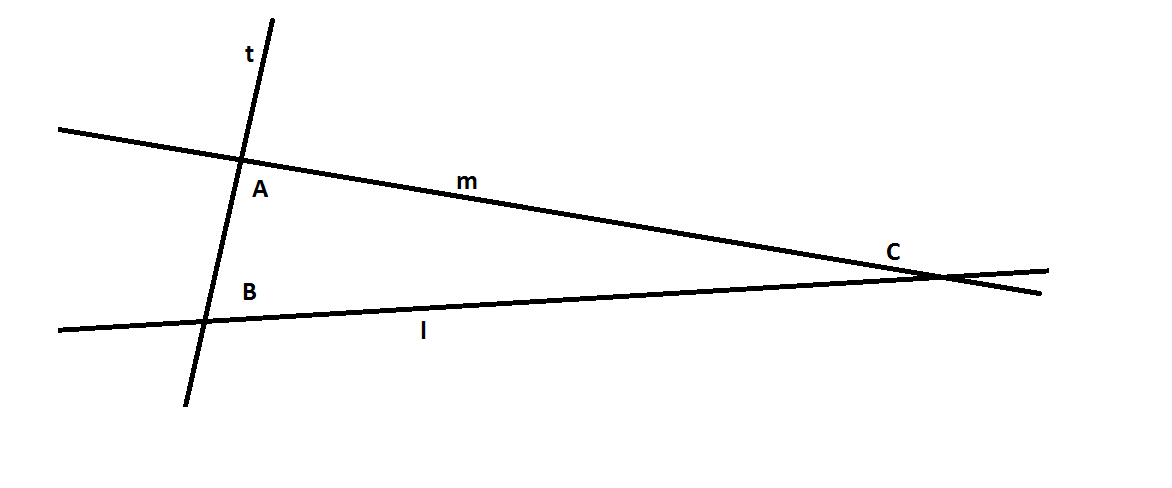
\includegraphics[width=4in]{hw5_prob1.png}
\end{center}

\QED





\prob{10} Prove proposition 4.7.  Deduce as a corollary that transitivity of parallelism is equivalent to Hilbert's Euclidean parallel postulate.\\

\noindent Proposition 4.7: Hilbert's Euclidean parallel postulate $\Leftrightarrow$ if a line intersects one of two parallel lines, then it also intersects the other. \\


\Proof

\noindent $\Rightarrow:$  Assume Hilbert's Euclidean parallel postulate and assume to the contrary that we have some line t that intersects $l\neq t$ where $l||m$ but t does not intersect m. Therefore $t || m$.    Additionally we know that t intersects l at some point, call it P.  By Hilbert Euclidean parallel postulate we know that there is at most one line through P parallel to m.  However we know that $P \in t$ and $t||m$ as well as $P \in l$, $l ||m$ yet we know that t and l are distinct.  Contradiction.  Therefore Hilbert's Euclidean parallel postulate implies the other statement.\\




\noindent $\Leftarrow:$ Assume that for any two parallel lines and a line that intersects one of them, that it intersects the other.  \\


Given a line l and a point P not on l, assume to the contrary that there are at least 2 (distinct) lines through P parallel to l, call them m and n.  \\

Since m is parallel to l and since m intersects n at P, we know by assumption that n intersects l.  Contradiction.  Therefore there is at most 1 line parallel to l through P.

\QED

Now we must show that transitivity of parallelism is equivalent Hilbert's Euclidean parallel postulate.\\

Note that the following is transitivity of parallelism:\\

If $l \parallel m$ and $m \parallel n$ then $l \parallel n$.  \\

Now note the contrapositive.  \\

If $l$ intersects $n$, then l intersects m or m intersects n.\\

Given lines $l || m$.  Then we know that if l intersects some line n then m intersects n.  This is the right side of the bi-conditional statement in proposition 4.7, so we know that Hilbert's Euclidean parallel postulate is equivalent to transitivity of parallelism.



\prob{15} Here is Legendre's lemma-- which is needed for his proof found in many texts, based on the Archimedean property of angles, that the angle sum of every triangle is $\leq 180^\circ$.  He got he idea for this from Euclid's construction in his incomplete proof of the exterior angle theorem.  Given $\triangle ABC$.  Let $D$ be the midpoint of BC.  Let E be the point on the ray opposite to $\overrightarrow{DA}$ such that $DE \cong DA$.  Prove that $\triangle AEC$ has the same angle sum as $\triangle ABC$ and that either $(\angle AEC)^\circ$ or $(\angle EAC)^\circ$ is $\leq (\angle BAC)^\circ$.  Hint see figure 4.29.  Use congruent triangles to show that $(\angle AEC)^\circ + (\angle EAC)^\circ = (\angle BAC)^\circ$.  \\

\Proof

By Proposition 3.15 we know that vertical angles are congruent so we know that $\angle BDA \cong EDC$.  Also since D is the midpoint of BC, we know that $BD \cong DC$ and the problem statement states that $AD \cong DE$.  By SAS we know that $\triangle BDA \cong CDE$.

Now we know that the angle sum of $\triangle ABC$ is 

\begin{eqnarray*}
\angle CBA^\circ + \angle ACB^\circ + (\angle BAC^\circ) &=& \angle CBA^\circ  + \angle ACB^\circ + (\angle BAD^\circ + \angle DAC^\circ) \text{ by angle addition}\\
&=& \angle CBA^\circ  + \angle ACB^\circ + (\angle CED^\circ + \angle DAC^\circ) \text{ by congruent triangles}\\
&=& \angle DBA^\circ  + \angle ACB^\circ + \angle CED^\circ + \angle DAC^\circ \text{ since $\overrightarrow{BD} = \overrightarrow{BC}$}\\
&=& \angle DCE^\circ  + \angle ACB^\circ + \angle CED^\circ + \angle DAC^\circ \text{ by congruent triangles}\\
&=& \angle DCE^\circ  + \angle ACB^\circ + \angle CED^\circ + \angle DAC^\circ \text{ by angle addition}\\
&=& (\angle DCE^\circ  + \angle ACD^\circ) + \angle CED^\circ + \angle DAC^\circ \text{ since $\overrightarrow{CD} = \overrightarrow{CB}$}\\
&=& (\angle ACE^\circ)  + \angle CED^\circ + \angle DAC^\circ \text{ by angle addition}\\
&=& \angle ACE^\circ  + \angle CEA^\circ + \angle DAC^\circ \text{ since $\overrightarrow{ED} = \overrightarrow{EA}$}\\
\end{eqnarray*}

which is the angle sum of $\triangle AEC$.

\QED


Use Legendre's lemma to give an RAA proof of the Saccheri-Legendre theorem.  Hint: repeat this construction enough times. \\

\Proof

Assume to the contrary that the angle sum of $\triangle ABC$ is greater than $180^\circ$.  Then we know that at least one of $\angle A, \angle B$, and $\angle C$ must have a degree measure greater than 60.  Without loss of generality, let $\angle C^\circ > 60^\circ$.

Then consider using the lemma.  So we bisect BC as before and make a new point E as above and make our new triangle, $\triangle ACE$.  Now we know by angle addition that $\angle ACE^\circ = \angle ACB^\circ + \angle BCE^\circ$.  From this we can see that if we keep bisecting the side connecting C and the new point of the triangle, the angle at point C in the new triangle will have angle measure equal to the previous triangle's angle measure for the angle associated with angle C and the angle associated with the new point. The reason for this is angle addition.  The two angles in our original triangle added together are $\angle ACB$ and $\angle DCE \cong \angle CBA$. After doing this procedure from the lemma, the angle associated with point C will repeatedly grow as we go to new triangles.  Additionally, if the angle associated with point A is greater than the other angle at some iteration (the other angle meaning the angle that is not associated with point A or C in some new triangle made by iterating this procedure), then we can bisect AC so we are added the larger angle to $\angle C$ at each iteration.  If we choose the larger angle to add to $\angle C$, then we are always adding half the difference between the angle sum of the triangle (the original, or by Lemma, any triangle in the sequence of iterations).  Remember that the triangle angle sum is $(180 + x)^\circ$, so each time we are adding at least $(\frac{180 + x - \angle C^\circ}{2})^\circ$, or in other words, the measure of $\angle C$ moves at least half way to $180 + x$ at each iteration.  By Real variables II and some calculus courses, we know we can keep repeating this and eventually $(\frac{180 + x - \angle C^\circ}{2})^\circ < x$ meaning that $\angle C^\circ > 180^\circ$, but this contradicts the definition of an angle. Hence a triangle's angle measure must be less than or equal to $180^\circ$.
 
\QED



\prob{19} Prove the theorem of Thales that in a semi-Euclidean plane, an angle inscribed in a semicircle is a right angle (see Figure 4.31).\\

\Proof

Given a semi Euclidean plane and an angle inscribed in a semi-circle in that plane.  Note, that by definition one side must go through the center of the circle, call the center O (otherwise we could easily have a equilateral triangle in the circle).  \\

By Saccheri's theorem, all triangles in the plane have angle measure sum of $180^\circ$ since it is semi-Euclidean.\\

Consider the triangle $\triangle ABC$ inscribed in the circle.  We know that $BO \cong AO \cong CO$ since they are all radii of the same circle (definition of circle).  By Proposition 3.10 we know therefore that $\angle B \cong \angle BAO$ and $\angle C \cong \angle CAO$ since the triangles are isosceles. Therefore by angle addition we know that $\angle BAO^\circ+ \angle CAO^\circ = \angle BAC^\circ$. Therefore let $\angle B^\circ = x$ and let $\angle C^\circ = y$. So we know that $2x + 2y = 180^\circ$, so $x+y = 90$.  However this is the measure for $\angle BAC$.  Therefore $\angle BAC$ is a right angle. 

\QED





\prob{20a} Find the flaw in the following argument purporting to construct a rectangle.  Let A and B be any two points.  There is a line l through A perpendicular to $\overleftrightarrow{AB}$ (Proposition 3.16)  and, similarly, there is a line m through B perpendicular to $\overleftrightarrow{AB}$. Take any point C on m other than B.  There is a line through C perpendicular to l-- Let it intersect l at D.  Then $\square ABCD$ is a rectangle.\\

Everything is fine until the assumption that the line perpendicular to l through C is perpendicular to m.  This makes the assumption that rectangles exist, which is what the author is trying to prove.


\prob{21} There sphere, with ``lines'' interpreted as great circles, is not a model of neutral geometry.  Here is a proposed construction of a rectangle on a sphere.  Let $\alpha, \beta$ be two circles of longitude and let themn intersect the equator at A and D.  Let $\gamma$ be a circle of latitude in the northern hemisphere intersecting $\alpha$ and $\beta$ at two other points, B and C.  Since circles of latitude are perpendicular to circles of longitude, the quadrilateral with vertices ABCD and sides the arcs of $\alpha, \gamma, \beta$ and the equator traversed in going from A north to B east to C south to D west to A should be a rectangle.  Explain why this construction doesn't work.\\

Note that the great circles of longitude meet at the north pole and that the further you get from the equator, the closer together the two great circles become.  Knowing this, opposite segments AD and BC will be of different length. 


\prob{28} A quadrilateral is convex if it has the property that each pair of opposite sides, say AB and CD, has the property that CD is contained in one of the half planes bounded by the line through A and B, and AB is contained in one of the half-planes bounded by the line through C and D.  Using Pash's theorem, prove that if one pair of opposite sides has this property, then so does the other pair of opposite sides. \\

\Proof

Suppose the pair AB, CD has the mentioned property.  So we know that $AB$ does not intersect $\overleftrightarrow{CD}$ and $CD$ does not intersect $\overleftrightarrow{AB}$.  \\

Suppose then that AD intersects $\overleftrightarrow{BC}$ at some point.  Call it E.  Since AD is distinct from AB and CD, $E\neq B$ and $E\neq C$ (if they held two points in common, they would be the same line, I1).  Therefore either $E*B*C$ or $B*C*E$ (definition of quadrilateral specifically states that segments cannot intersect except at the endpoints). Without loss of generality, let us say that $E*B*C$. \\ 

Consider the triangle $\triangle DEC$. Now since $E*B*C$ we know that $\overleftrightarrow{AB}$ intersects EC at B.  Therefore by Pasch's theorem, $\overleftrightarrow{AB}$ must also intersect either DE or DC, call this new point F.  If it intersects on DE, then $\overleftrightarrow{AB}$ has A and F in common with AD, which is not permitted as this is a quadrilateral.   Therefore $\overleftrightarrow{AB}$ must intersect DC.  Contradiction by assumption. \\


\QED





\prob{9}  You will show in Exercise 16 that the following statement can be proved in Euclidean geometry:  If points P,Q,R lie on a circle with center O, and if $\angle PQR$ is acute, then $(\angle PQR)^\circ = \frac{1}{2} (\angle POR)^\circ$.  In neutral geometry show that this statement implies the existence of a triangle whose angle sum is $180^\circ$.


Assume that given 3 points on a circle, the above property about angle measures hold.  Then let P and R lie on a circle in such a way that PR is not a diameter. 

Consider the triangle $\triangle POR$.  Notice that $PO$ and $OR$ are both radii of the circle, so we have an isosceles triangle, so by proposition 3.10 we know that $\angle ORP \cong \angle OPR$.  Therefore, bisect PR and call the midpoint S, so $PS \cong SO$.  Additionally we know that $OS \cong OS$.  So by SSS $\triangle OSP \cong \triangle OSR$.  Therefore we know that $\angle OSP \cong \angle OSR$, so they are both right angles.  Therefore, suppose that $\angle SPO^circ \geq 90$.  Then we know that since $\angle POR^\circ > 0$, that the angle measure of $\triangle POR$ is greater than $180^\circ$.  However, by Saccheri Legendre we know that this cannot be so.   Therefore $\angle SPO^\circ < 90$. However we know that we can construct an right angle here such that the new ray will be pointed into the circle.  We know this ray will intersect the circle, call this point Q.  

Using the assumption we have made, designate the following angle measures $\angle POR^\circ = 2x$ and $\angle PQR^\circ = x$.   By our earlier statements we know that $\angle RPQ^\circ = 90$ and by angle addition we know that $\angle RPO^\circ + \angle OPQ^\circ = 90$.  However we know that $PO \cong OQ$ since both are radii, and we know that $\angle OPQ \cong \angle OQP$ by proposition 3.10 (isosceles triangle) and we know $\angle OQR \cong SOP$ as their measure is both x (measurement theorem). Since angle congruence is transitive we know that $\angle OPQ \cong \angle SOP$ and we know that $\angle SPO^\circ + \angle OPQ^\circ = 90$ so we know that $\angle SPO^\circ + \angle SOP^\circ = 90$.  Additionally we know that $\angle OSP ^\circ = 90$ so the angle measure of $\triangle OPS$ is $180^\circ$. 

\begin{center}
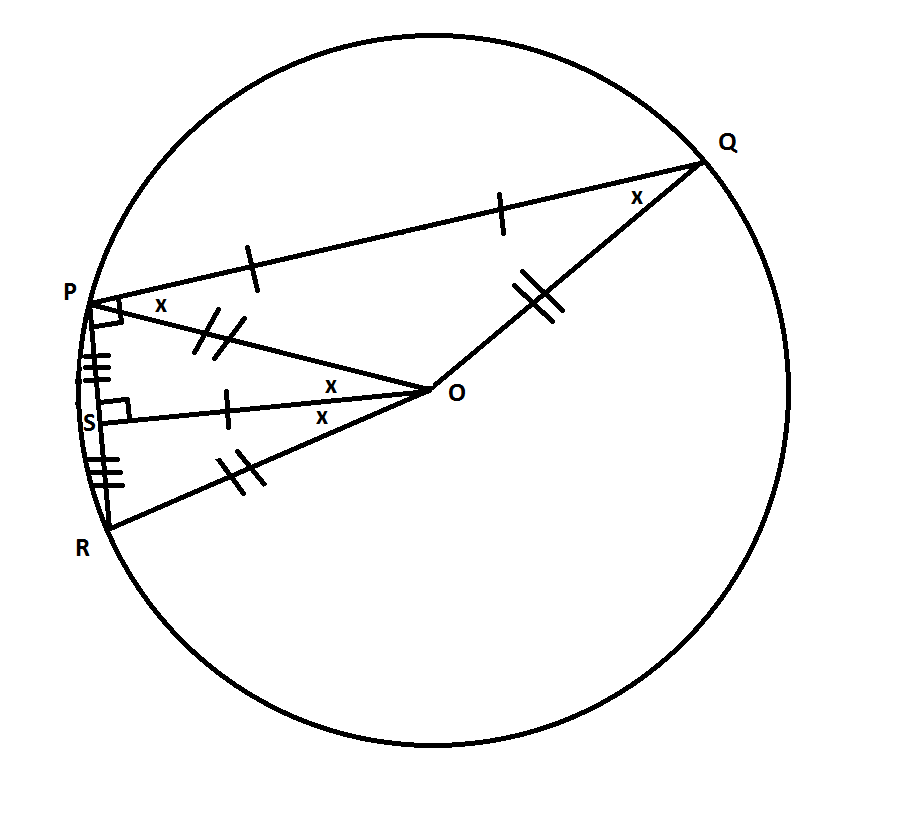
\includegraphics[width=4in]{hw5_prob9.png}
\end{center}
\QED



\end{document}